\section{Analysis}

\subsection{Methodology}

First, we aimed to build a simple predictive model that integrates the image data with the metadata measurements, with the goal of outperforming the metadata alone.
Comparison of SVM regressor (SVR), Elastic Net, Decision Tree, Random Forest, XGBoost, Voting, and Stacking (combining SVR, ElasticNet, Decision Tree, Random Forest, and XGBoost with the secondary model as indicated in the tables below) models were performed on the datasets.
A randomized grid search was performed separately for each model to determine the optimal hyperparameters before comparing the models.
Metrics such as Mean Squared Error (MSE), Root Mean Squared Error (RMSE), R-squared (R\textsuperscript{2}) were used as key evaluators.

Next, we built models on the integrated metadata and image data aiming for better performance but applying a PCA transformation on the image data, preserving 95\% of the variance.
As a result, the dimensionality of the image data was reduced from 4,096 pixels to 340 dimensions

Finally, we explored a Convolutional Neural Network (CNN) model to further enhance our predictive performance.
The CNN model is designed to automatically learn relevant features from the otolith images, which is particularly useful in identifying the age-related annuli in the images.
The CNN architecture used in this analysis consists of several convolutional and pooling layers, followed by fully connected layers that allow for regression of the fish age.

\subsubsection{CNN Model Architecture}

The CNN architecture used in this analysis includes:

\begin{itemize}
    \item \textbf{Convolutional Layers:} These layers apply filters to extract features from the images. We started with 32 filters in the initial layers, progressively increasing to 128 filters in the deeper layers.
    \item \textbf{Max-Pooling Layers:} These layers downsample the feature maps, reducing the computational load and aiding in generalization.
    \item \textbf{Flatten and Dense Layers:} The feature maps are flattened and passed through fully connected layers to predict the fish age.
    \item \textbf{Dropout Layer:} A dropout layer was incorporated to mitigate overfitting during training by randomly disabling a fraction of neurons.
\end{itemize}

The model was trained using the Adam optimizer and Mean Squared Error (MSE) as the loss function.
We evaluated the model's performance using key metrics such as Mean Squared Error (MSE), Root Mean Squared Error (RMSE), and R-squared (R\textsuperscript{2}) on both the validation and test datasets.

\subsection{Results}

In Table~\ref{tab:simple_models}, the results of simple models based on the reduced pixels and metadata are displayed.
The stacking (gradient boost) model is the top performer for metadata, with the lowest MSE (1.385594), the lowest RMSE (1. 177113), and the highest R\textsuperscript{2} (0.848093).
Other ensemble models, such as Stacking (linear regression), Random Forest, XGBoost, and Voting, performs similarly well in terms of accuracy, with MSE below 1.5, RMSE below 1.25, and an R\textsuperscript{2} above 0.83, slightly lower than the Stacking (gradient boost) model.
Single models, such as SVR, Elastic Net, and Decision Tree lag behind the ensemble methods in model performance.
Among them, the linear regression model Elastic Net shows drastically lower scores in evaluation metrics.

In Table~\ref{tab:pca_models}, we see the results from the PCA transformed data.
Stacking (Linear regression) model is the top performer for metadata, with the lowest MSE (1. 514197), the lowest RMSE (1. 230527), and the highest R\textsuperscript{2} (0. 833993).
Similar to the models built on the metadata alone, we observed that the ensemble models outperformed the single models.
Additionally, integrating image data improved the performance of some single models, particularly for the SVR and ElasticNet models.
Incorporating image data did not significantly improve the performance of the ensemble models as we had initially expected.

Finally, the results of the CNN test and validation set are displayed in Table~\ref{tab:cnn_models}.
The CNN model achieved an R\textsuperscript{2} of 0.73 on the test set, which is a promising result given the complexity of the task.
The model demonstrated a MSE of 2.64 and RMSE of 1.62, indicating room for improvement, but also showing that it performs better than simple models based solely on metadata.
The model showed better performance on the test set compared to the validation set, where the R\textsuperscript{2} dropped to 0.55.
A graph of the actual verse predicted ages of otolith images are displayed in Figure~\ref{fig:actual_vs_predicted}.
Further tuning of the model, such as experimenting with more complex architectures or adjusting hyperparameters, may improve performance on both the validation and test sets.

\pagebreak

\begin{figure}
    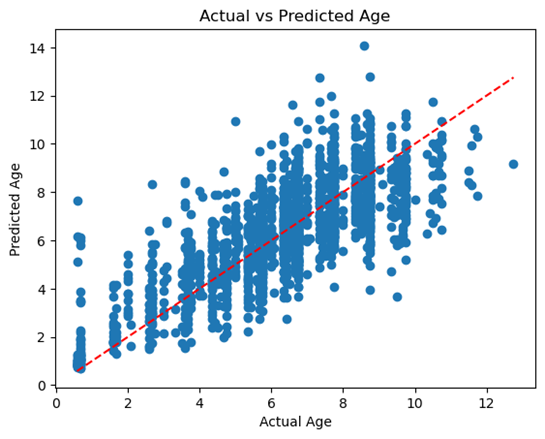
\includegraphics[width=\linewidth]{predict_vs_actual}
    \caption{Actual verses CNN predicted ages of otolith images}
    \label{fig:actual_vs_predicted}
\end{figure}



\pagebreak
\begin{longtable}{| p{.25\textwidth} | p{.25\textwidth} | p{.25\textwidth} | p{.25\textwidth} |}
    \caption{Performance summary of model built on metadata}
    \label{tab:simple_models} \\
    \hline
    \textbf{Model} &
    \textbf{Mean Squared Error \newline(MSE)} &
    \textbf{Root Mean Squared Error \newline (RMSE)} &
    \textbf{R-squared (R\textsuperscript{2})} \\
    \hline
    \hline
    SVR &
    1.984 &
    1.40864 &
    0.782458 \\
    \hline
    ElasticNet &
    2.104611 &
    1.450728 &
    0.769264 \\
    \hline
    Decision Tree &
    1.579715 &
    1.256867 &
    0.82681 \\
    \hline
    Random Forest &
    1.39943 &
    1.182975 &
    0.846576 \\
    \hline
    XGBoost &
    1.484482 &
    1.218393 &
    0.837251 \\
    \hline
    Voting &
    1.496319 &
    1.223241 &
    0.835953 \\
    \hline
    Stacking \newline(Linear regression) &
    1.391861 &
    1.179772 &
    0.847405 \\
    \hline
    Stacking \newline(Gradient boost) &
    1.385594 &
    1.177113 &
    0.848093 \\
    \hline
\end{longtable}

\pagebreak
\begin{longtable}{| p{.25\textwidth} | p{.25\textwidth} | p{.25\textwidth} | p{.25\textwidth} |}
    \caption{Performance summary of model built on integrated metadata and image data}
    \label{tab:pca_models} \\
    \hline
    \textbf{Model} &
    \textbf{Mean Squared Error \newline(MSE)} &
    \textbf{Root Mean Squared Error \newline (RMSE)} &
    \textbf{R-squared (R\textsuperscript{2})} \\
    \hline
    \hline
    SVR &
    1.774 & 683
    1.33217 & 2
    0.805435 \\
    \hline
    ElasticNet &
    1.858366 &
    1.363219 &
    0.796261 \\
    \hline
    Decision Tree &
    1.766926 &
    1.329258 &
    0.806286 \\
    \hline
    Random Forest &
    1.558563 &
    1.248424 &
    0.829129 \\
    \hline
    XGBoost &
    1.587466 &
    1.259947 &
    0.825961 \\
    \hline
    Voting &
    1.547636 &
    1.24404 &
    0.830327 \\
    \hline
    Stacking \newline(Linear regression) &
    1.514197 &
    1.230527 &
    0.833993 \\
    \hline
    Stacking \newline(Gradient boost) &
    1.614702 &
    1.270709 &
    0.822975 \\
    \hline
\end{longtable}


\pagebreak
\begin{longtable}{| p{.25\textwidth} | p{.25\textwidth} | p{.25\textwidth} | p{.25\textwidth} |}
    \caption{Performance summary of model built on integrated metadata and image data}
    \label{tab:cnn_models} \\
    \hline
    \textbf{Dataset type} &
    \textbf{Mean Squared Error \newline(MSE)} &
    \textbf{Root Mean Squared Error \newline (RMSE)} &
    \textbf{R-squared (R\textsuperscript{2})} \\
    \hline
    \hline
    Test &
    2.64 &
    1.62 &
    0.73 \\
    \hline
    Validation &
    2.13 &
    1.46 &
    0.55 \\
    \hline
\end{longtable}

